\documentclass[]{article}
\usepackage[]{algorithm2e}
\usepackage{amsmath}
\usepackage{framed}
\usepackage{tabularx}
\usepackage[dutch]{babel}
\usepackage{graphicx}
\usepackage{mcode}

%opening
\title{Practicum NMB : Eigenwaardenproblemen}
\author{Matthijs van Keirsblick en Harald Sch\"{a}fer}
\date{vrijdag 25 april 2014}

\newcommand{\opgave}[1]{\section*{Opgave #1}}


\begin{document}

\maketitle
\opgave{1}

We beginnen door een QR-factorisatie te berekenen van $A_{0}$ met eender welke methode. Vervolgens berekenen we $b = Q^{*}*b_{0}$. Met deze waarden kunnen we de iteratieve berekening starten die hieronder beschreven staat. De $G_{x}$ matrices zijn givens transformaties om de toegevoegde rijen van K terug op nul te stellen om zo terug een bovendriehoeksmatrix R te bekomen waarin de nieuwe waarden in verwerkt zijn.

\begin{framed}
\begin{algorithm}[H] 
 $Q^{(0)}*R^{(0)} = A_{0}$\\
 $b = Q^{(0)*}*b_{0}$\\
 \For{i = 1 to k}{
  $f = n*d$\\
  $R^{(i)} = G_{f}^{*}*...*G_{1}^{*}*
  \begin{bmatrix}
    	R^{(i-1)}	\\
    	K
    \end{bmatrix}$\\
  $R^{(i)} = R^{(i)}(:n,:)$\\
  $Q^{(i)} = I*G_{1}*...*G_{f} $\\
  $b^{(i)} = Q^{(i)*}*
  \begin{bmatrix}
      	b^{(i-1)}	\\
      	c
      \end{bmatrix}$\\
  $b^{(i)} = b^{(i)}(:n,:)$\\
 }
 
% \caption{How to compute incremental least squares solution with QR factorisation}
\end{algorithm}
\end{framed}

Aan het einde van elke iteratie is het mogelijk om $x^{(i)}$ te berekenen door achterwaardse substitutie toe te passen op de vergelijking $R^{(i)}*x^{(i)} = b^{(i)}$. Omdat na elke iteratie maar $R^{(i)}$ en  $b^{(i)}$ opgeslagen moet worden is het duidelijk dat het gebruikte geheugen niet toeneemt. Omdat de grootte van de matrices R en b niet toeneemt neemt het rekenwerk ook niet toe met elke iteratie. Voor het berekenen van een Givens-transformatie zijn 2 delingen, 2 vermenigvuldigen, een optelling en een vierkwantswortel nodig. Er moeten n*d Givens-transformaties berekend worden per iteratie. Een vermenigvuldiging met een rotatiematrix van grootte n+d zoals in dit geval vraagt 4*(n+d) vermenigvuldigingen en 2*(n+d) optellingen. Er gebeuren 2*n*d -1 van die matrix vermenigvuldiginge per iteratie. Tot slot  gebeurt er nog voor de berekening van de $b^{(i)}$ een matrix vermenigvuldiging waarvoor $(n+d)^2$ vermenigvuldigingen gebeuren en $(n+d-1)^2$ optellingen.

\begin{itemize}
  \item $n*d*2$ delingen
  \item $n*d$ vierkantswortels
  \item $n*d*2 + 2*(n+d)*(2*n*d-1) + (n+d-1)^2 \approx 4*n^2*d$ optellingen
  \item $n*d*4 + 4*(n+d)*(2*n*d-1) + (n+d)^2 \approx 8*n^2*d$ vermenigvuldigingen
\end{itemize}

%\section{}

\opgave{3}
Alvorens de QR methode, al dan niet met shifts, toe te passen op de matrix, moeten we hem omzetten naar Hessenberg vorm. Deze omzetting kost ons \'{e}\'{e}nmaal \textit{O}($n^3$) rekenwerk. \linebreak
Omdat de Hessenberg vorm al bijna bovendriehoeks is, kan de QR factorisatie in minder stappen uitgevoerd worden, namelijk in \textit{O}($n^2$) in plaats van in \textit{O}($n^3$). Deze factorisatie moet in iedere iteratie van de QR methode uitgevoerd worden, dus  de vermindering in rekenwerk is erg significant. 

\begin{figure}
\begin{center}
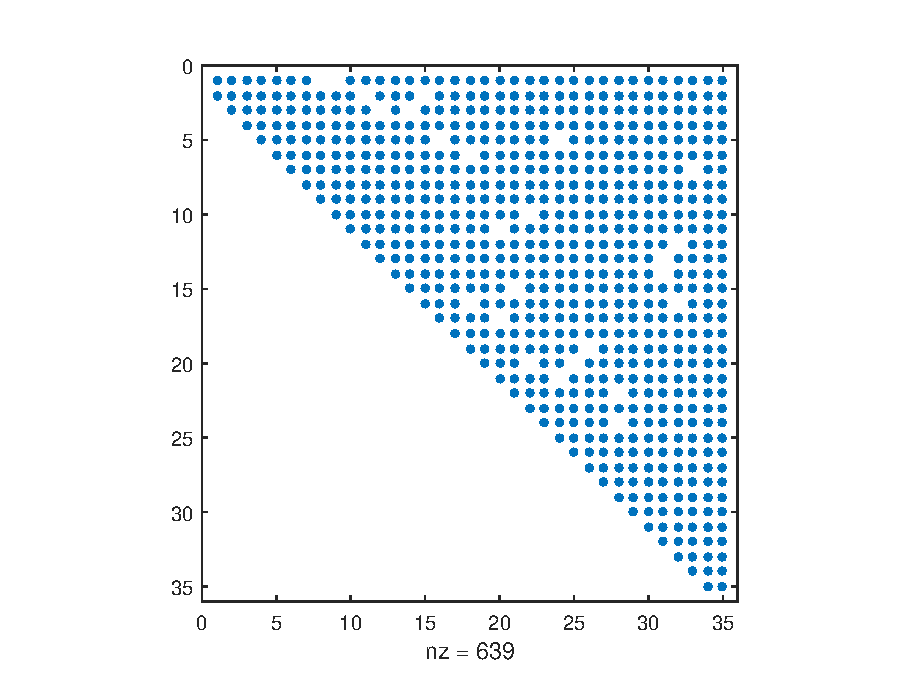
\includegraphics[width=1\textwidth]{opgave3.eps}
\end{center}
\caption{Opgave 3: De structuur van de Hessenberg- vorm van mat1}
\end{figure}

\opgave{4}

De verwachting vanuit de theorie is dat de QR methode zonder shifts traag convergeert, zoals power- iteratie. De QR methode met shifts zou in het slechtste geval niet(Rayleigh shifts) of kwadratisch (Wilkinson shifts) convergeren. Hieronder worden het benodigde aantal iteratiestappen per methode in grafiek- en tabelvorm weergegeven, samen met de fout op het tussenliggende resultaat. We merken op dat  zowel de Rayleigh Shift als de Wilkinson Shift zorgen voor een kubische convergentie (aantal beduidende cijfers $* 3$ in iedere stap). 
De Wilkinson Shift heeft in dit geval een snellere convergentie door een (toevallig) goedgekozen eerste shiftwaarde. De convergentiefactor voor de eerste stap van de Wilkinson shift methode is hier $3.46$, voor de Rayleigh shift methode is hij $2.827$ en voor de QR methode zonder shift is hij zelfs kleiner dan 1. Het valt op dat de QR methode zonder shift niet lijkt te convergeren op deze grafiek. Dit is wel zo, maar pas na een groot aantal stappen (niet weergegeven). Na ~40 iteratiestappen is de machinenauwkeurigheid bereikt. 

\begin{figure}
\begin{center}
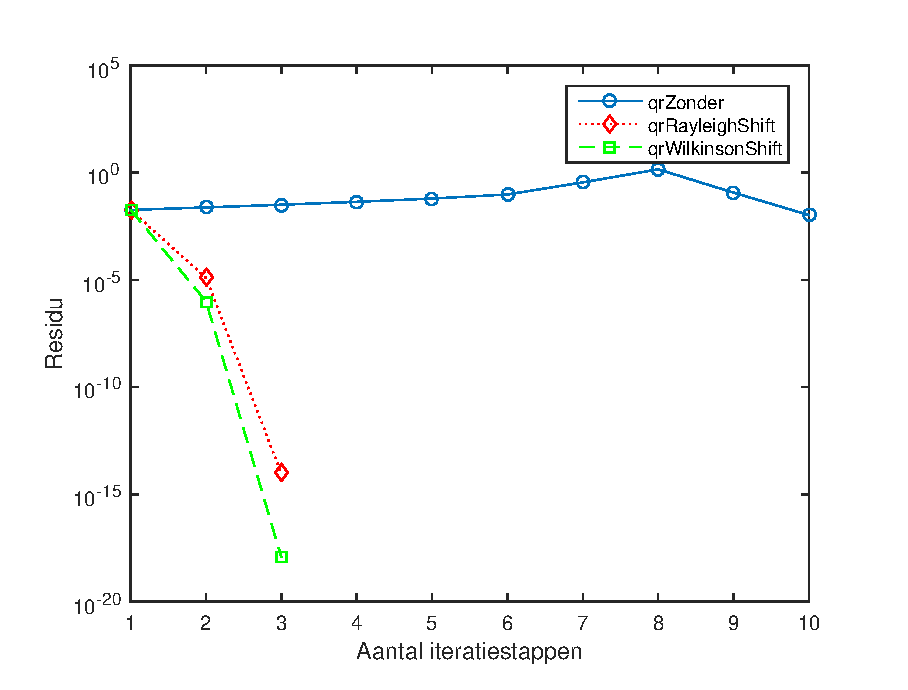
\includegraphics[width=1\textwidth]{opgave4.eps}
\end{center}
\caption{Opgave 4: De fout op het berekenen van \'e\'en eigenwaarde.}
\label{figuurtje}
\end{figure}

\begin{table}
\noindent\makebox[\textwidth]{%
\begin{tabularx}{1.3\textwidth}{l|llllllllll}
Methode&1&2&3&5&10&20&25\\\hline
QRzonder&$0.01836$ & $0.02411$ & $0.03212$ & $0.06223$ & $0.0106$ & $1.498\times 10^{-6}$ & $2.059\times 10^{-8}$ \\
QRrayleigh & $0.01836$ & $1.234\times 10^{-5}$ & $\epsilon_{mach}$ & $\epsilon_{mach}$ & $\epsilon_{mach}$ & $\epsilon_{mach}$ & $\epsilon_{mach}$ \\
QRwilkinson & $0.01836$ & $9.833\times 10^{-7}$ & $\epsilon_{mach}$ & $\epsilon_{mach}$ & $\epsilon_{mach}$ & $\epsilon_{mach}$ & $\epsilon_{mach}$\\
\end{tabularx}}
\caption{convergentie QR methodes voor eigenwaardenberekening}
\label{tabelOpgave4}
\end{table}

\paragraph{•}
Een aantal zaken zijn nog op te merken:
\begin{itemize}
	\item Voor de 2 methoden die gebruik maken van shifts, wordt in iedere stap een aantal keren een geshifte inverse iteratie gedaan, om zo het element op positie $(k,k)$ te laten convergeren naar de $k-de$ eigenwaarde. Opmerkzaam is dat de $i-de$ eigenwaarde met $i = 1,\dots,k-1$ als k het aantal eigenwaarden is dat we nog moeten berekenen, ook al genaderd wordt, terwijl het algoritme nog bezig is eigenwaarden verderop in de matrix te berekenen m.b.v shift- iteraties. Hoe kleiner i, hoe minder sterk dit effect. De oorzaak hiervan is dat de QR methode, naast inverse iteratie, ook simultane iteratie toepast.
	\item De methode met Wilkinson- shifts doet er 66 stappen over om alle eigenwaarden van mat1 te vinden tot op machineprecisie. De methode met Rayleigh- shifts doet er 83 stappen over, en die zonder shifts maar liefst 686 stappen. Wilkinson shifts zijn beter dan de Rayleigh shifts, omdat zij rekening houden met het symmetrische eigenwaarden. Rayleigh shifts kunnen in zo'n gevallen zorgen voor een trage (of zelfs onbestaande) convergentie.
\end{itemize}


\opgave{8}

Algemene werkwijze om met de bisectiemethode de k-de eigenwaarde $\lambda_k$ te vinden van een symmetrische, tridiagonale matrix A van grootte m:

\begin{enumerate}
 \item Kies een interval $I=[a0,b0]$ dat $\lambda_k$ bevat.
 \item Dan geldt, gebruik makende van de Sturm sequentie en de interlace- eigenschap van eigenwaarden van opeenvolgende submatrices $A_{i:,i:}$ van A, : $s(b_0) >= k$ and $s(a_0) < k$ met s het aantal tekenwisselingen in de sequentie. Hieraan moet steeds voldaan zijn. Door $b_0$ en $a_0$ te verkleinen of vergroten kunnen we het interval I laten convergeren naar de waarde van $\lambda_k$.
 \item Gebruik de bisectietechniek om het interval te verkleinen: evalueer de Sturm sequentie $p_k(a_0) = det(A^{(k)} - a*I)$ voor $k=1\dots m$ waarbij $a=(a0+b0)/2$, en tel het aantal tekenwisselingen $s$. Als \'{e}\'{e}n van de sequentiewaarden 0 is, vergelijk je de volgende waarde met de laatste waarde die niet 0 was. Voor Matlab-code, zie hieronder.
 \item Als $s >= k$, vervang $b_0$ door $(a0+b0)/2$ en herhaal de iteratie, maar nu op het kleiner interval $I=[a_0,(a0+b0)/2]$.
 Indien $s < k$, vervang $a_0$ door $(a0+b0)/2$ en herhaal.
 \end{enumerate}
 Door herhaalde iteratie en verkleinen van het inverval convergeert het algoritme naar de k-de eigenwaarde van A. Een aantal grafieken van de convergentie naar de echte eigenwaarden zijn weergegeven in ~\ref{opgave8.eps}
 
 Om nu alle eigenwaarden binnen een interval te bekomen, moeten we vinden welke eigenwaarden zich binnen dit interval bevinden.Met behulp van de Sturm sequentie en de interlacing eigenschap van de submatrices van A, kunnen we bepalen hoeveel eigenwaarden er zijn in het interval I. Het aantal eigenwaarden in het interval $ (- \ inf, a_0]$ is gelijk aan het aantal tekenveranderingen in de Sturm sequentie $ p_k (a_0) = det (A ^ {(k)} - A0 * I) $, met k=1\dots m als m de grootte is van de matrix A. De index van de eerste eigenwaarde in het interval is dan dit getal + 1. Op dezelfde manier kunnen we het aantal eigenwaarden kleiner dan $ b_0 $ bepalen. Het aantal eigenwaarden in het interval $ \ links (a_0, b_0 \ right) $ is dan het verschil tussen de twee. We kennen dus de indices van eerste en laatste eigenwaarden in het interval I, en kunnen voor al deze indices het hierboven beschreven algoritme toepassen.

\begin{framed}
\begin{lstlisting}
function [E,residue,nbSteps] = bisection(A,a,b,tol)
% Eigenvalue of tridiagonal matrix using the bisection method
%   A       The matrix 
%   a       The lower bound of the interval
%   b       The upper bound of the interval
%   tol     The precision with which to determine the eigenvalues

%   E       The column vector with resulting eigenvalues
%   residu  The matrix with residues after each step, one row per
%   eigenvalue calculation

[p,sBeforeA0] = sturmSeq(A,a);
[p,sBeforeB0] = sturmSeq(A,b); 
 % sBeforeA0 = number of eigvals before the interval, 
 % so first eigval in interval has index sBeforeA0 + 1
nbEigInterval = sBeforeB0 - sBeforeA0;
E = zeros(nbEigInterval,1);
residue = zeros(nbEigInterval,1);
nbSteps = zeros(nbEigInterval,1);

n = size(A,1);
eigA = eig(A);

for k=sBeforeA0+1:sBeforeB0
    % bisection for locating k'th eigenvalue
    xl = a; %   lower bound
    xu = b; %   upper bound
    i = 1;  %   used for the residue
    exactLambda = eigA(k); %    this too
    x= rand(n,1);          %    this too
    
    while xu-xl >= tol
        xn = (xl+xu)*.5;
        i = i+1;
        [p,s] = sturmSeq(A,xn); % sturmSeq with shift xn, 
        						% returns nb_eigenvalues in (-inf, xn)
        residue(k - sBeforeA0,i) = norm(exactLambda*x - xn*x);
        
        if s >= k       % you counted too much, 
        				% so it's located in the first half of the interval
            xu = xn;
        else            % not enough eigvalues found yet, 
        				% search in second half of the interval
            xl = xn;
        end
    end
    
    E(k - sBeforeA0) = xn;    %save calculated eigenvalues
    nbSteps(k - sBeforeA0,1) = i;
end
\end{lstlisting}
\label{matlabBisection}
\end{framed}



\begin{framed}
\begin{lstlisting}
function [ p,s ] = sturmSeq( A, shift )
% This function returns the sequence of det(A - xI) 
% and the number of sign changes
%   A = tridiagonal matrix
%   lamb = guess eigen value (used in bisection method)
%   p = a pvector polynomials (p_1 to p_n)
%   s = the number of sign changes

n= size(A,1);
p = zeros(n,1);
s = 0; 
prevsign= 1; %p(0) = 1

% p(-1) = 0 & p(0) = 1
p(1) = (A(1,1) - shift) * 1 - 0^2 * 0;  
if sign(p(1))*prevsign < 0
    s = s+1; 
    prevsign = - prevsign;
end

p(2) = (A(2,2) - shift)*p(1) - A(1,2)^2 * 1;
if sign(p(2))*prevsign < 0
    s = s+1; 
    prevsign = - prevsign;
end

% for the rest, we can just use the formula
for k = 3:n
    % A(k,k) = a_k ; A(k,k-1) = b_k-1  because b_k-1 is the entry on 
    % the k-1'th column of row k, and a_k is the k-th entry on that row 
    % (b is offdiagonal element, a is diagonal element)
    p(k) = (A(k,k) - shift)*p(k-1) - A(k-1,k)^2 * p(k-2);     %formula (30.9)
    if sign(p(k))*prevsign < 0 
        s = s+1; 	% sign change means new eigenvalue found 
        			% in interval (-inf,shift)
        prevsign = - prevsign;
    end
end
\end{lstlisting}
\label{matlabSturm}
\end{framed}

\begin{figure}
\begin{center}
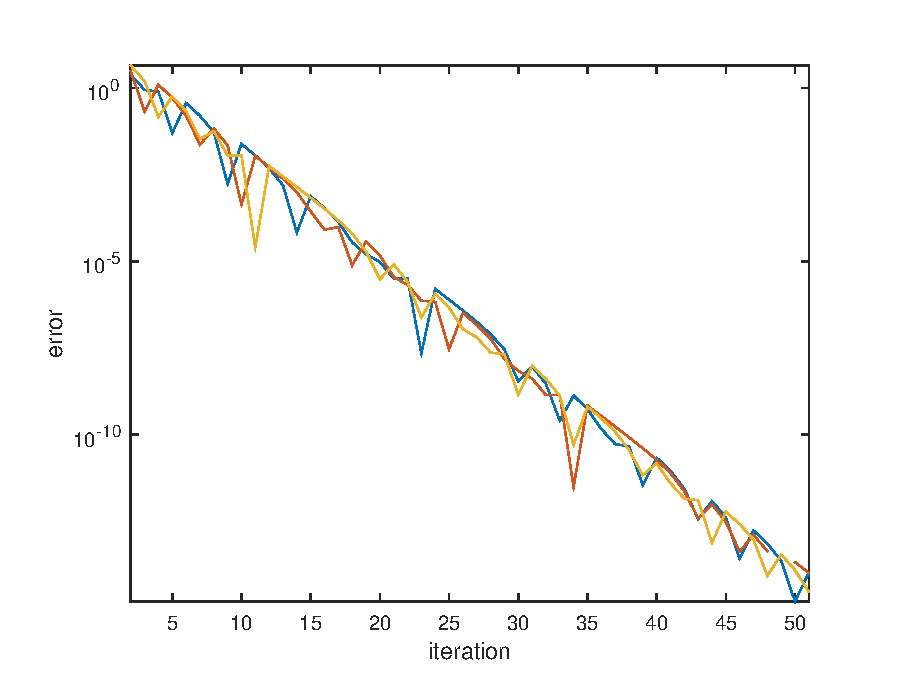
\includegraphics[width=1\textwidth]{opgave8.eps}
\end{center}
\caption{Opgave 8: De evolutie van het residu bij het berekenen van een aantal eigenwaardes}
\label{opgave8}
\end{figure}


Tests ter controle van de werking van deze Matlab- functies zijn hieronder weergegeven. In alle gevallen waarin de methode convergeert, gebeurt dit 
\begin{itemize}
	\item Een diagonale matrix met 5 gelijke eigenwaarden. Het algoritme vindt ze allemaal. Bij grote matrices van deze vorm worden vrij grote benaderingsfouten gemaakt voor de ide eigenwaarden. Bij de $i$-de eigenwaarde is de fout 2 keer zo groot als bij de $(i-1)$-de eigenwaarde.
	A\[\left[ \begin{array}{cccccc}
6 & 0 & 0 & 0 & 0 \\  
0 & 6 & 0 & 0 & 0 \\  
0 & 0 & 6 & 0 & 0 \\ 
0 & 0 & 0 & 6 & 0 \\ 
0 & 0 & 0 & 0 & 6 \\  
\end{array} \right] \]\linebreak

	\item Een diagonale matrix met allemaal verschillende positieve elementen. Bij  grotere matrices (vanaf ongeveer grootte 100) van deze vorm kunnen de opeenvolgende $p_i$'s zo in absolute waarde stijgen, dat ze na een tijd niet meer voorgesteld kunnen worden in de computer (er is geen compenserende factor $b_{k-1}^2$ in formule (30.9) in het HB, omdat de buitendiagonaalelementen allemaal nul zijn). Het algoritme vindt dan niet alle eigenwaarden.

	\item Een willekeurige matrix, die dus niet tridiagonaal is, zelfs niet symmetrisch. De bissectie methode werkt hier inderdaad niet, zoals door de theorie voorspeld.
\[	\left[	\begin{array}{ccccc}
0.88058&0.82562&0.15711&0.88857\\
0.23512&0.88369&0.62517&0.26367\\
0.24486&0.94537&0.69899&0.23479\\
0.64092&0.3908&0.085869&0.83966\\
\end{array}	\right]	\]\linebreak

	\item Een matrix die bijna tridiagonaal is, behalve \'{e}\'{e}n element. De bissectie methode werkt hier inderdaad niet, zoals door de theorie voorspelt.
	\[ \left[	\begin{array}{llllll}
3&6&0&0&0&0\\
6&3&1&0&0&0\\
0&1&3&2&0&0\\
0&0&2&3&3&0\\
0&0&0&3&3&4\\
5&0&0&0&4&3\\
\end{array}	\right] \]

	\item Gewone symmetrische tridiagonale matrices, met het zoekinterval van verschillende groottes, positief/negatief,...

\end{itemize}

\end{document}
